\documentclass{article}
\pdfpagewidth=8.5in
\pdfpageheight=11in

\usepackage{ijcai19}

% Use the postscript times font!
\usepackage{times}
\usepackage{soul}
\usepackage{url}
\usepackage[hidelinks]{hyperref}
\usepackage[utf8]{inputenc}
\usepackage[small]{caption}
\usepackage{graphicx}
\usepackage{amsmath}
\usepackage{booktabs}
\usepackage{tocloft}
\usepackage{url}
\urlstyle{same}

% dot leaders for section entries in table of contents
\renewcommand{\cftsecleader}{\cftdotfill{\cftdotsep}}

\newcommand{\etal}{\textit{et al.}}

\title{Is attention really all you need?}

\author{
Kyle Roth\\
\affiliations
Brigham Young University\\
\emails
kylrth@gmail.com
}

\begin{document}

\maketitle

\tableofcontents

\vspace{30px}

\begin{abstract}
This is a wonderful abstract.
\end{abstract}

\section{Introduction}

The attention mechanism is an exciting development in the artificial intelligence community. The concept is simple, and rooted in our understanding of attention in biological intelligence \cite{glimpses,neuroscience-inspired}. Attention mechanisms also lend themselves to more intuitive interpretation, an attractive feature as concerns about model interpretability gain traction. In this review, we observe the trajectory that current research is taking with regard to the theory and application of attention, and suggest where future work with attention may yield fruits. [STRENGTHEN THIS THESIS]

\subsection{Background on neural machine learning}

Machine learning is a branch of artificial intelligence that deals with training a model to perform tasks by providing the model with data. There are various types of machine learning algorithms, applicable to different tasks. One of the most popular algorithms is the neural network. A neural network is a system of connections between simple functions (e.g. multiplication, summation, ReLU \cite{relu}), which together approximate a larger, more complex function. It has been proven that sufficiently large neural networks can approximate arbitrary continuous functions \cite{universal_approximators}. Theoretically, this means that for every reasonable mapping there exists a neural network that replicates it. Some example mappings are listed in Table~\ref{table:mappings}.

\begin{table}
    \centering
    \begin{tabular}{|c|c|}
        \hline
        \textbf{Input} & \textbf{Output} \\
        \hline
        images & the objects the image contains \\
        \hline
        audio recordings & a text transcription \\
        \hline
        English text & a French translation \\
        \hline
    \end{tabular}
    \caption{The caption of the table}\label{table:mappings}
\end{table}

Most commonly, neural networks undergo supervised training, meaning that they are shown the correct output for each training example and made to improve in some way. Neural networks generally use backpropagation and gradient descent to train weights that are present in the simple functions of the network. Backpropagation uses the difference between the correct example and the network's output to determine how the weights in the network need to change. Figure~\ref{figure:backpropagation} provides a visualization of backpropagation in a neural network.

\begin{figure}
    \centering
    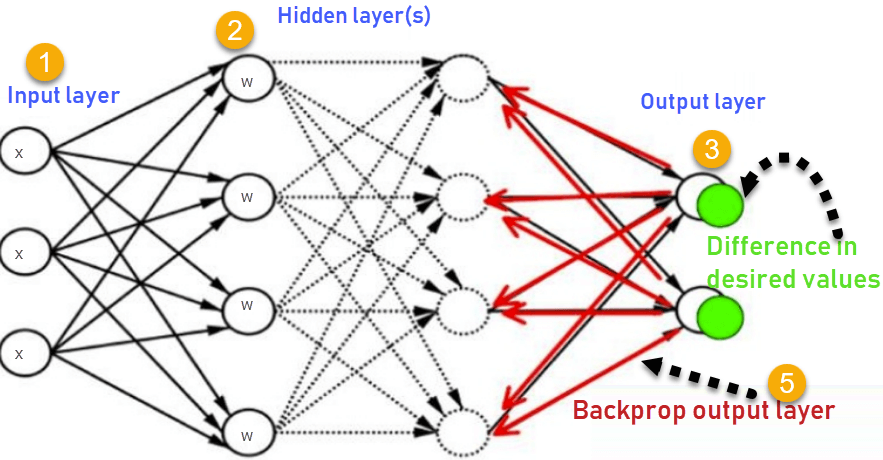
\includegraphics[width=3in]{figures/backpropagation.png}
    \caption{A visualization showing that backpropagation uses the difference between the desired and actual output to train the weights of the neural network. Image source~\protect\cite{backprop}.}\label{figure:backpropagation}
\end{figure}

While the theoretical limitations of neural networks are quite permissive, it is relatively difficult to train them. Backpropagation is sensitive to ``noisy'' or incorrect data, meaning that data selection is at least as important as architecture selection. The training process is also relatively expensive in terms of computation time and memory usage; neural networks are commonly trained for days or even months \cite{attn_all_you_need}.

Another real issue is that backpropagation is unlikely to find the ``global optimum'', the absolutely optimal set of weights that approximate the function. This is due to the fact that the algorithm only adjusts the weights incrementally, and can get stuck in a ``local optimum'', a condition where no slight change would improve performance but performance is still not as good as at the global optimum.

These difficulties with training neural networks are the reason that so much effort is given to developing better network architectures. Certain architectures and data representations lend themselves to a smoother search space for the weights, increasing the likelihood that backpropagation reaches a better optimum.

\subsection{Description of attention}

Attention appears to provide that smoother search space for training the network because its output can explicitly depend on each input given to the network, while also giving an intuitive view of the inputs that the network learns to ``attend'' to.

Bahdanau \etal~[\citeyear{joint_align_translate}] first described attention as an ``alignment model'' for words in a sentence to be translated. They used an RNN encoder-decoder model as others had before \cite{encoder_decoders}, but for every position in the target sentence, the alignment model produced a ``soft alignment''\footnote{In machine translation, alignment refers to the pairing of words or phrases in the source sentence with words or phrases in the target sentence.} between the target location and every word in the source sentence. See Figure~\ref{figure:rnn_search} for more details on the model.

The key development here was the use of a soft alignment, meaning that each pair of source and target words was given an alignment score between 0 and 1. This made the alignment calculation differentiable, allowing the alignment to be performed by a feed-forward neural network trained along with the rest of the model.

\begin{figure}
    \centering
    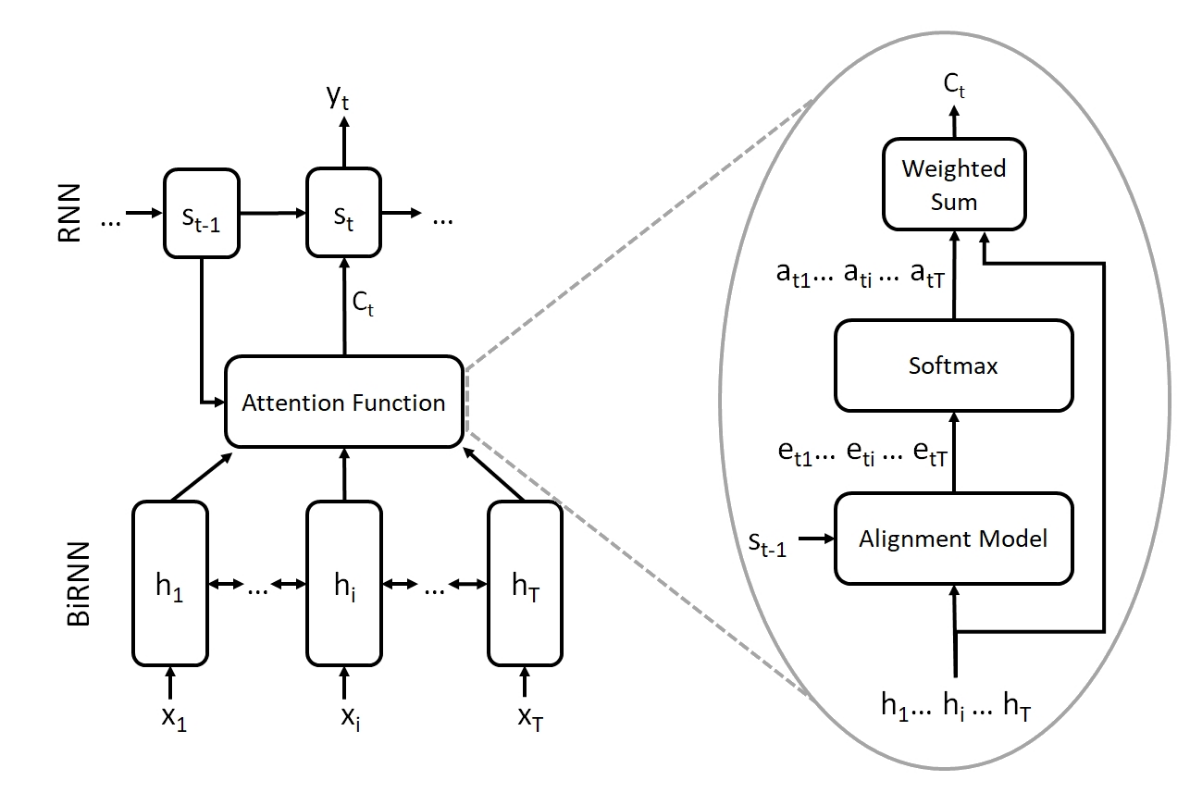
\includegraphics[width=3in]{figures/rnn_search.png}
    \caption{The model used by \protect\cite{joint_align_translate}. They used a bidirectional RNN to encode each word $x_i$ into a fixed-length vector $h_i$. Then, for every position $t$ in the target sentence, the alignment model produced an alignment vector $a_t$, a measure of alignment between the target location and every word in the source sentence. $a_t$ was used to find the weighted sum $c_t=\sum_{i=1}^Ta_{ti}h_i$, which was used as the input to the decoder (a unidirectional RNN). Note that the alignment model also received the previous decoder RNN state $s_{t-1}$ as input. Image source~\protect\cite{attention_please}.}\label{figure:rnn_search}
\end{figure}

\section{Theoretical generalization}

Ironically, attention mechanisms have received lots of attention since their conception in \citeyear{joint_align_translate}. Initially formulated as a word alignment mechanism for text translation \cite{joint_align_translate}, the concept was expanded [BY WHOM? SEE WHO CITES THESE GUYS]

\cite{listen_attend_spell}

Unsure: \cite{show_observe_tell}, \cite{draw}

\subsection{Self-attention}

\cite{self_attentive_embedding}

\subsection{Attention between existing pairs}

\cite{natural_language_inference}

\subsection{Attention on arbitrary graphs}

\cite{graphs}

\subsection{Attention as a lookup}

\subsection{Active memory}

\cite{active_memory}

Neural memory resources aren't the same thing \cite{neural_turing}?

\section{Application}

\subsection{Attention without recurrent layers}

\cite{attn_all_you_need}

\section{Interpretation}

Can you use attention to do feature importance?

\section{Conclusion}


\bibliographystyle{named}
\bibliography{main}

\end{document}
